Im Paper werden zwei unterschiedliche Daten erhoben. Es wurden echte GPS-Daten
gewonnen, die einen natürlichen Fehler unterliegen, als auch korrekte
Sensordaten, die mit künstlichen Fehler im nachhinein versehen wurden. Im
Folgenden betrachten wir ausschließlich GPS-Daten, deren Ergebnisse auch auf
die Sensordaten gelten.
\\\\
Die GPS-Daten sind durch eine Person mit einem Smartphone erhoben worden, der eine
festgelegte Strecke zurücklegte. Aufgrund der bekannten Strecke lassen sich
markierte Werte gewinnen. Hierbei wurde festgestellt, dass 186 von 742
Datenpunkte fehlerhaft sind. In der Abb.~\ref{gps} liegt ein Beispiel für einen
Fehler von GPS-Daten vor.  Zwischen den Datenpunkte 400 und 500 bewegte sich
die Person relativ nah an einem hohen Gebäude, sodass die durch den Smartphone
gewonnen Datenpunkte unzuverlässig sind. Vergleicht man die unterschiedlichen
State-of-art Methoden mit den neu entwickelten IMR, dann lässt sich
feststellen, dass IMR die Reparatur signifikant verbessert. 


\begin{figure}[htbp]
    \centering
    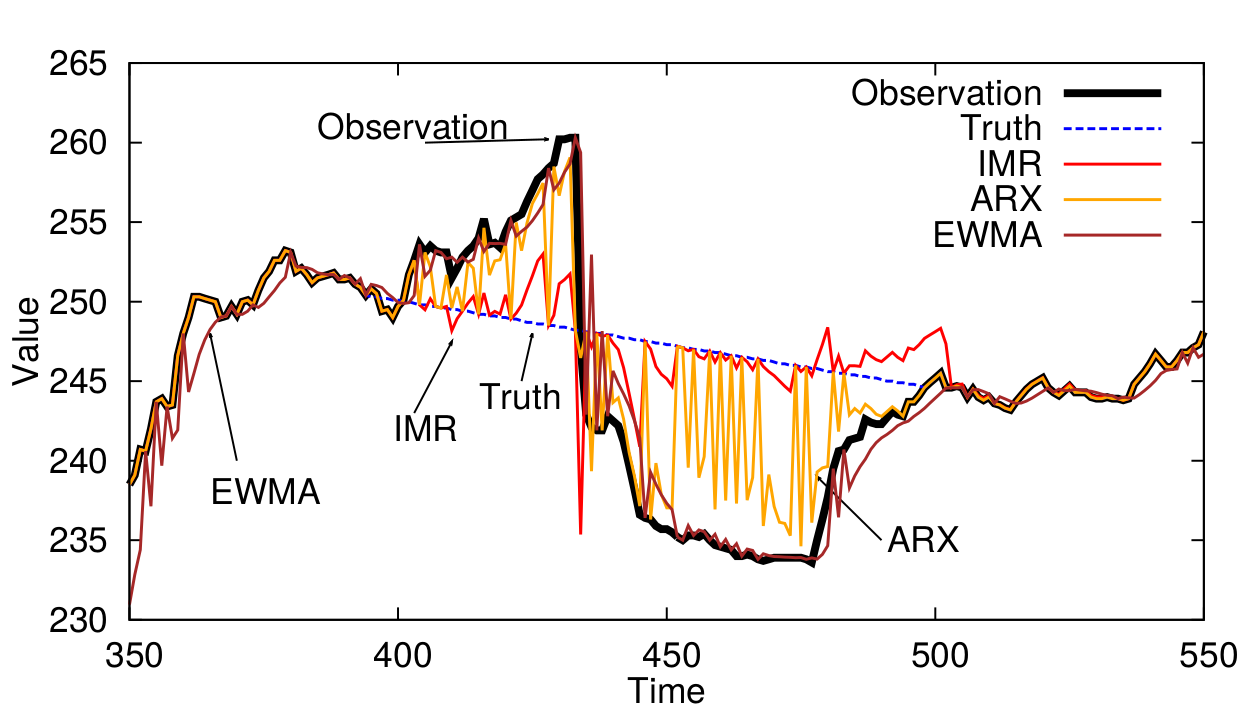
\includegraphics[width=\textwidth]{../plots/gps_example.png}
    \caption{Beispiel eines GPS-Fehler aus den Messungen.}%
    \label{gps}
\end{figure}
~\\
Im folgenden werden unterschiedliche Einstellungen der Verfahren als auch
unterschiedliche Einstellungen der gegebenen Daten vorgenommen. Neben den
Vergleich der betrachteten Verfahren lassen sich auch Rückschlüße ziehen,
inwiefern IMR für eine gute Performance eingestellt werden soll.

\subsection{Vergleich mit unterschiedlicher Ordnung}
\begin{figure}[htbp]
    \centering
    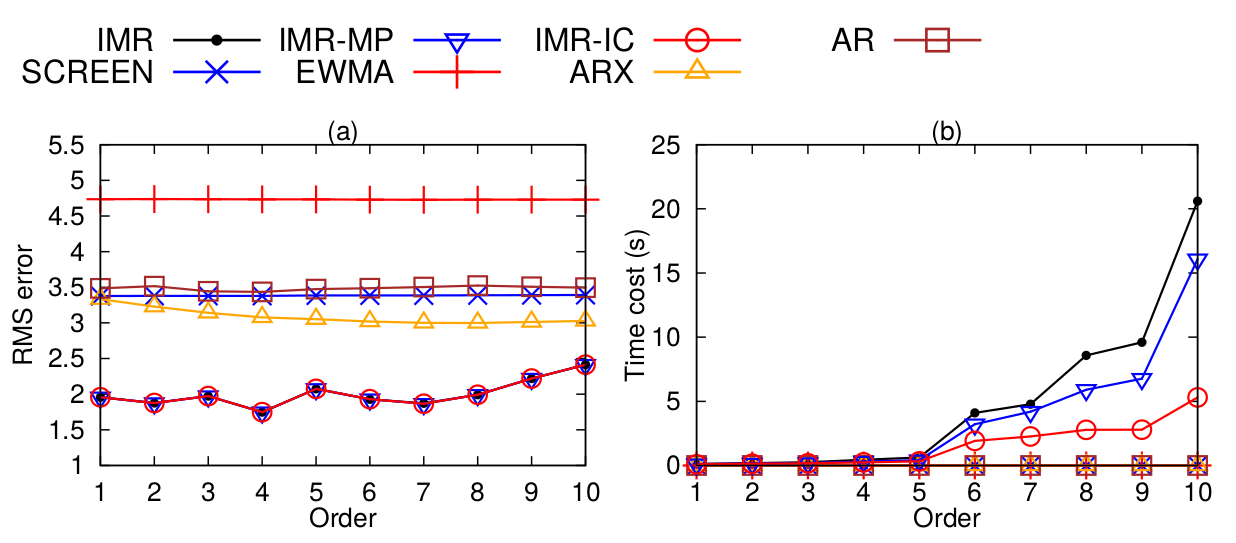
\includegraphics[width=\textwidth]{../plots/varying_order_p.png}
    \caption{Unterschiedliche Ordnung $p$ über GPS-Daten mit $\tau$ = 0.2, Datengröße 750 und Markierungsrate 0.2}%
    \label{varying_order_p}
\end{figure}

In der Abb.~\ref{varying_order_p} sind die Messergebnisse für verschieden
Ordnungen $p$ gegeben. Da die Verfahren EWMA und Screen keiner Ordnung
zugrundeliegen, sind die Messwerte über die Ordnung $p$ konstant. Dabei lässt
sich feststellen, dass EWMA stets schlechtere Ergebnisse als alle andere
Verfahren liefert. Screen hingegen kann auch mit steigender Ordnung mit AR(p)
und ARX(p) konkurrieren. Aufgrund von der einfachenen Modellannahme von AR(p),
ARX(p) und IMR(p) und der Datengröße werden auch bei steigender Ordnung die
Reparatur nicht besser. Interessant scheint hier zu sein, dass IMR bei der
Ordnung $p=4$ das beste Ergebnis erzielt, jedoch ab diesen Punkt der RMS-Fehler
schlechter wird. In der rechten Teilabbildung lässt sich erkennen, dass IMR(p)
mit steigender Ordnung einen exponentiellen Anstieg der Laufzeit zugrundeliegt.
Dabei verbessern die optimierten Version die Laufzeit erheblich. IMR-IC ist in
diesen Fall die bessere Wahl. Insgesamt lässt sich keine genaue Aussage über
die Wahl der Ordnung $p$ treffen, weil der RMS-Fehler sich nicht signifkant
verbessert oder verschlechtert, wohingegen die Laufzeit stark zunimmt. Daher
ist der Fall $p=1$ für den Online-Algorithmus als unterschungswert einzustufen.

\subsection{Vergleich mit unterschiedlichen Schwellenwerte}
In der Abb.~\ref{varying_threshold} wird der Effekt des Metaparameters $\tau$
dargestellt. $\tau$ erzeugt ein Trade-off zwischen Genauigkeit (niedrige
RMS-Fehler) und Laufzeit. Man kann in dem selben Bild erkennen, wie die drei
Varianten von IMR die gleiche Genauigkeit für unterschiedliche Schwellenwerte
besitzen. Jedoch bei einem Schwellenwert kleiner als $0.5$ IMR-IC zeigt eine
niedrigere Laufzeit.  Des Weiteren wird ein kleineren Reparaturfehler mit ein
niedrigen $\tau$ erreicht. Ein konservatives Reparation der Daten erfordert
dazu eine längere Rechenzeit. 
\begin{figure}[htbp]
    \centering
    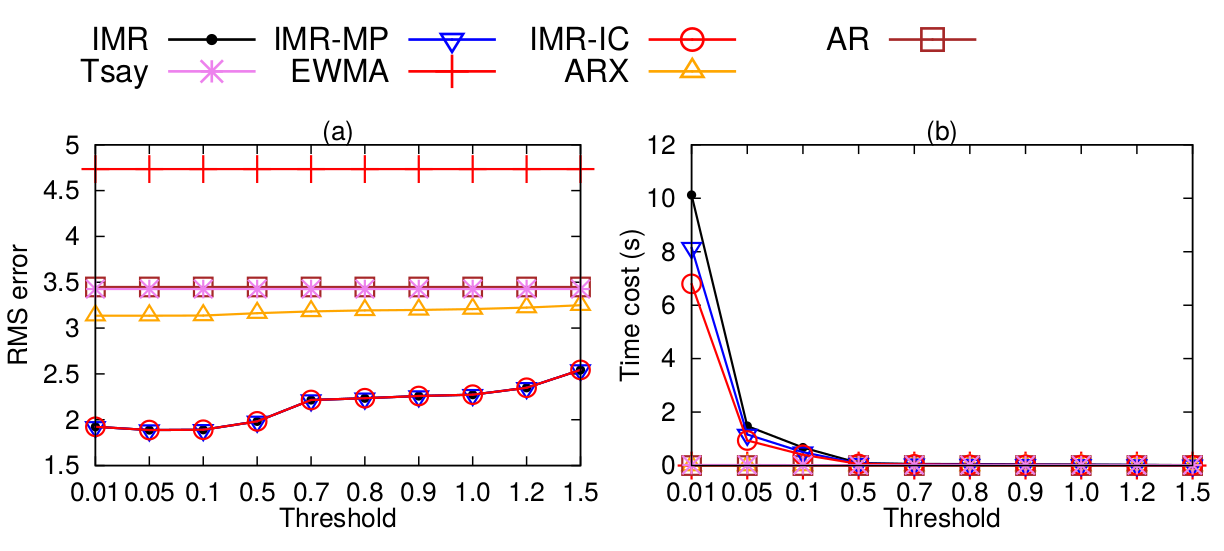
\includegraphics[width=\textwidth]{../plots/varying_threshold.png}
    \caption{Unterschiedliche Schwellenwerte $\tau$ über GPS-Daten mit $p$ = 3, Datengröße 750 und Markierungsrate 0.2}%
    \label{varying_threshold}
\end{figure}
\subsection{Vergleich mit unterschiedlichen Max. Anzahl von Iterationen}
Es gibt zwei Bedingungen in\ref{alg:imr} um aus der Schleife zu brechen: eine
feste programmierte maximale Anzahl von Iterationen und nach der Konvergenz von
$y^{(k)}$ mit $y^{(k-1)}$. Der Abb.\ref{varying_threshold} zeigt wie IMR schon
nach ein paar Tausende Iterationen eine relativ höhe Genauigkeit erreicht, die
sogar Konvergiert. Natürlicherweise steigt die Laufzeit von IMR linear mit der
Nummer von Iterationen hoch.
\begin{figure}[htbp]
    \centering
    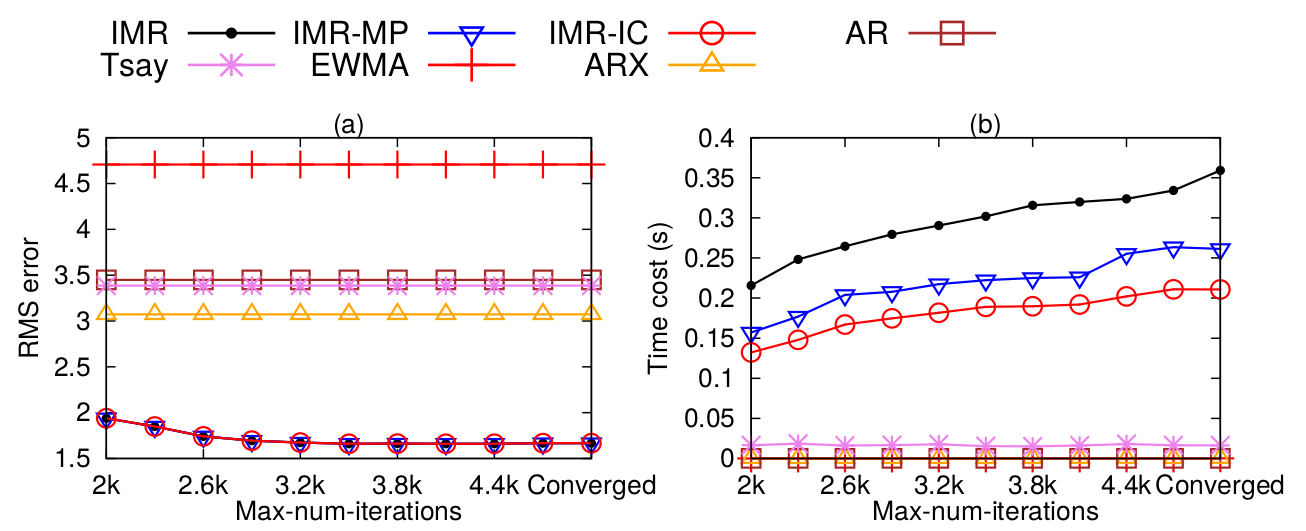
\includegraphics[width=\textwidth]{../plots/varying_maximum_number.png}
    \caption{Unterschiedliche maximale Anzahl von Iterationen über GPS-Daten mit $\tau = 0,2$, $p$ = 3 und Datengröße 750}%
    \label{varying_maximum_number}
\end{figure}
\subsection{Vergleich mit unterschiedlichen Markierungsraten}

In der Abb.~\ref{varying_labeling_rate} sind die Messergebnisse für
verschiedene Markierungsraten angegeben. Es wurden die Markierungsraten 0.01
bis 0.5 betrachtet. Wenn die Markierungsrate 0.1 beträgt, dann sind 10 \% der
Daten markiert. Man erwartet hier, dass ARX und IMR die besseren Ergebnisse
erzielen, da sie die Abweichung von Messwert zu markierten Werten besser
ausnutzen als die anderen Verfahren. Jedoch führt eine hohe Markierungsrate
ebenfalls zu einer Verbesserung der anderen Algorithmen, da sie direkt in die
Reparatursequenz einfliessen. Diese Hypothesen spiegeln sich auch in der
Abbildung ab. Ein bemerkenswerter Punkt ist hier die Laufzeit von IMR. Bei
steigender Markierungsrate nehmen die Laufzeitkosten zu und erreichen ein
Maximum bei ungefähr der Markierungsrate von 0.15. Bei einer zu geringen
Markierungsrate terminiert IMR schneller, weil es die meisten Messungen als
Reparatur übernimmt. Bei einer zu hohen Markierungsrate konvergiert IMR
ebenfalls schneller, da wenige Datenpunkte eine Reparatur erfordern. 

\begin{figure}[htbp]
    \centering
    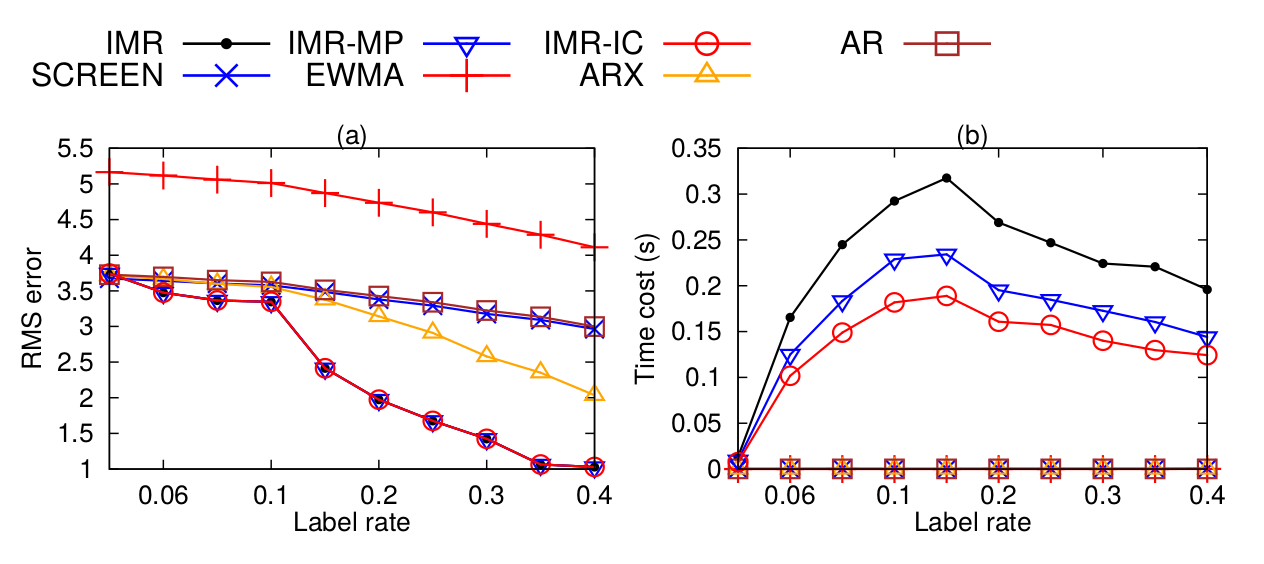
\includegraphics[width=\textwidth]{../plots/varying_labeling_rate.png}
    \caption{Unterschiedliche Markierungsraten über GPS-Daten mit $\tau = 0,2$, $p$ = 3 und Datengröße 750}%
   \label{varying_labeling_rate}
\end{figure}
